\chapter{Result Tables}

\section{Passive Haptics Experiment}
\label{sec:app_ph_exp}

\subsection{Ballistic Filter Histograms}
\label{sec:app_ph_metrics}

\begin{figure}[H]
    \centering
    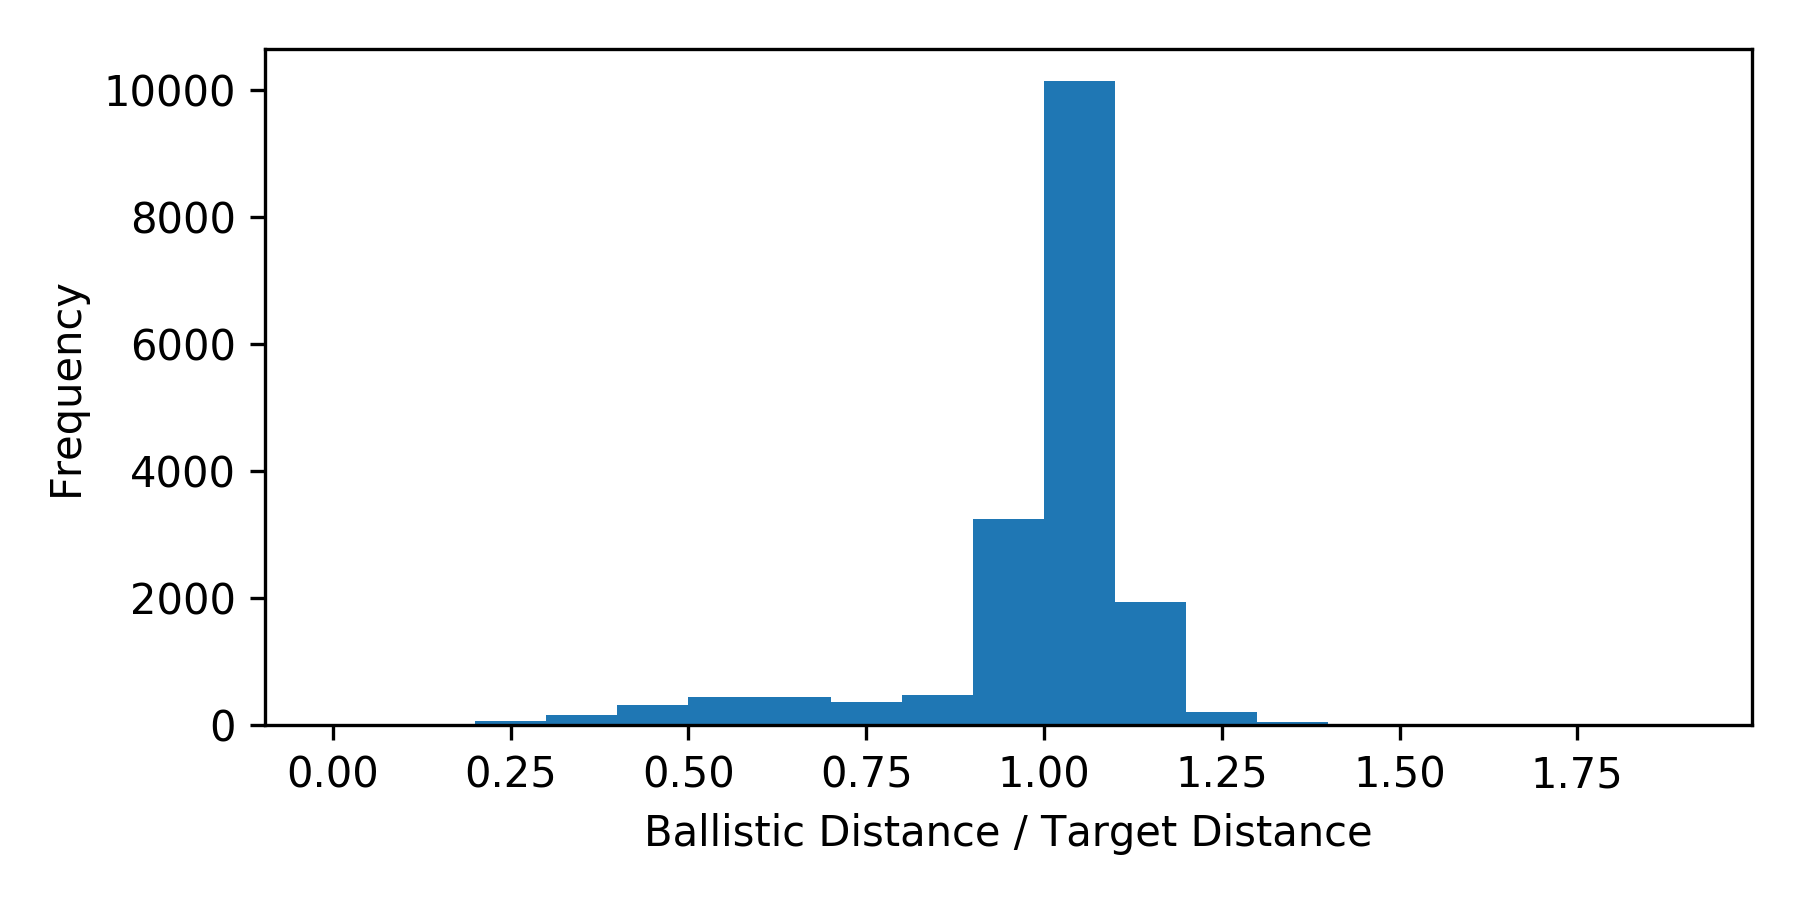
\includegraphics[width=\textwidth]{target_histogram.png}
    \caption{Ballistic Filter Histogram: Ballistic Distance over Target Distance. Movements below 0.90 and above 1.10 were filtered out.}
    \label{fig:ph_histogram_target}
\end{figure}

\begin{figure}[H]
    \centering
    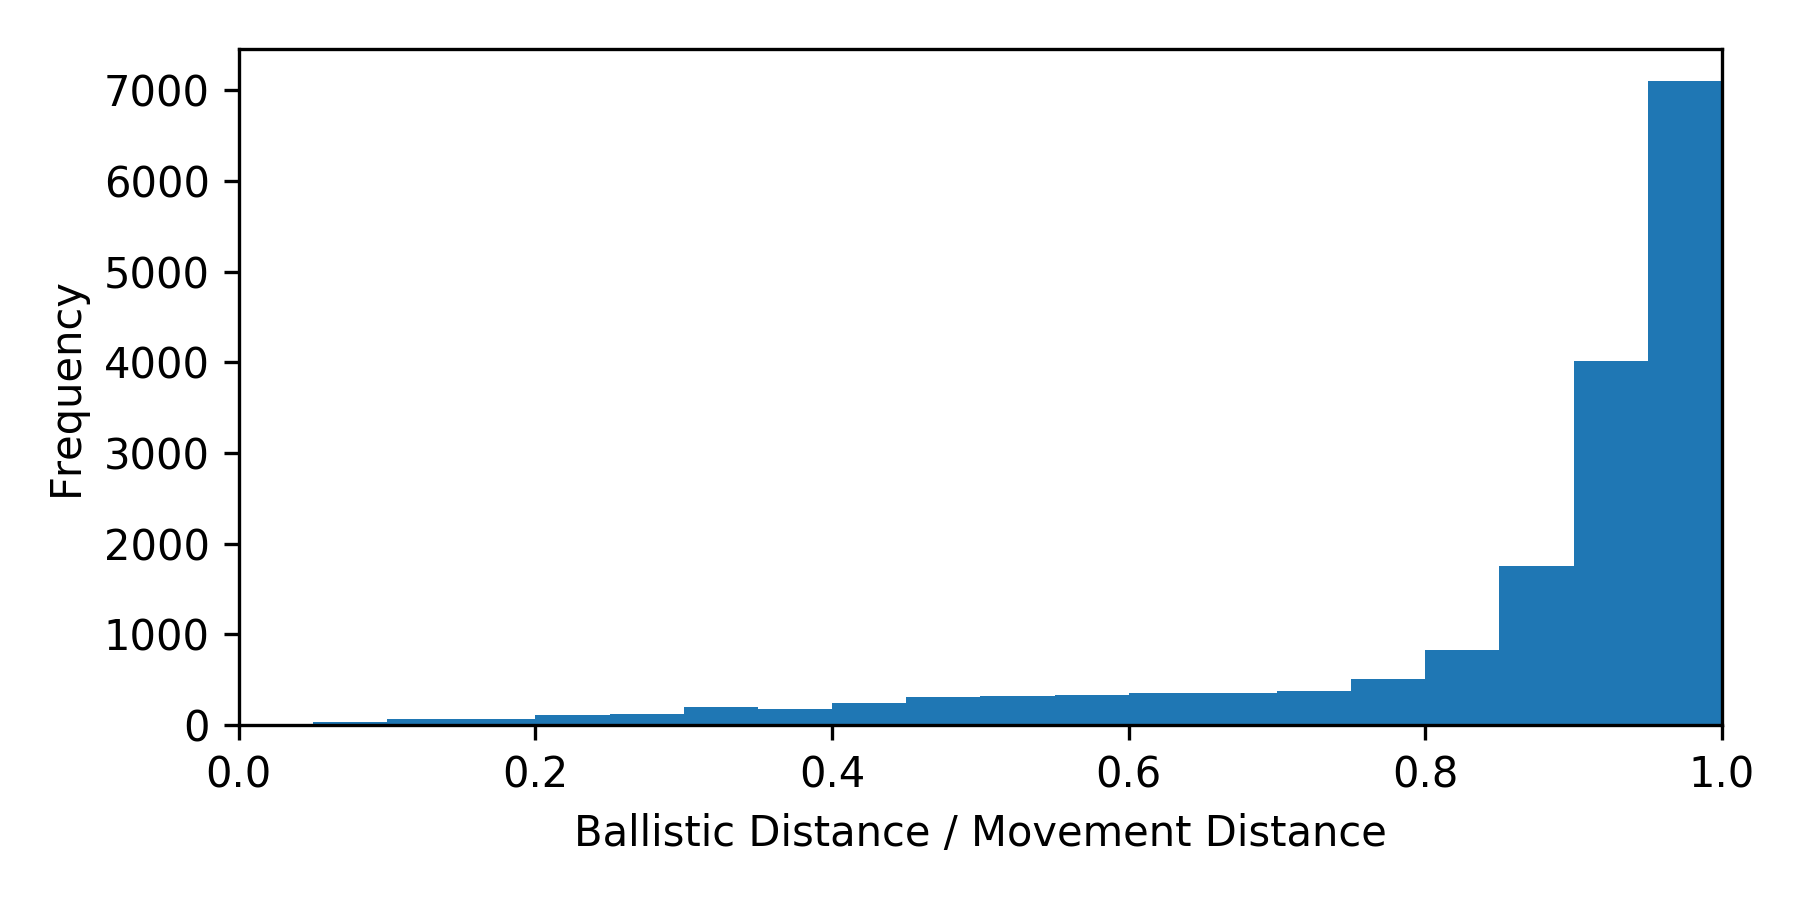
\includegraphics[width=\textwidth]{distance_histogram.png}
    \caption{Ballistic Filter Histogram: Ballistic Distance over Movement Distance. Movements below 0.80 were filtered out.}
    \label{fig:ph_histogram_distance}
\end{figure}

\begin{figure}[H]
    \centering
    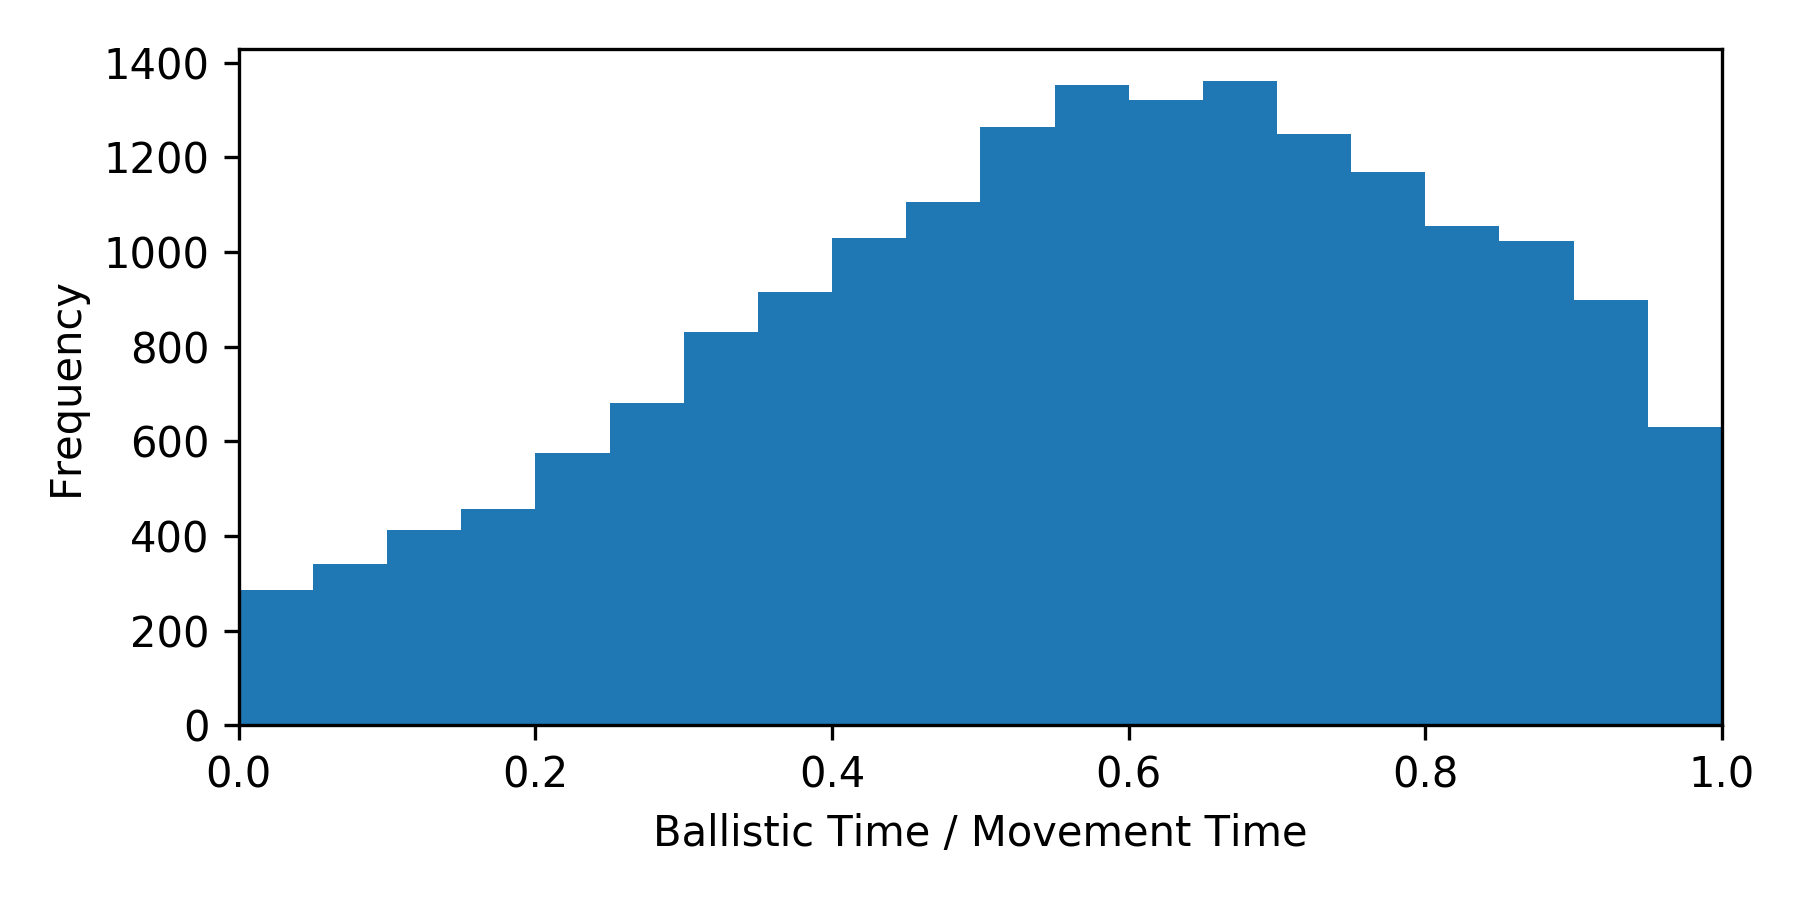
\includegraphics[width=\textwidth]{time_histogram.png}
    \caption{Ballistic Filter Histogram: Ballistic Time over Movement Time. Movements below 0.40 were filtered out.}
    \label{fig:ph_histogram_time}
\end{figure}

\subsection{Statistical Tables}

\begin{table}[H]
    \centering
    \includetable{throughput_means.tex}
    \caption{Throughput Means}
    \label{tab:ph_throughput_means}
\end{table}

\begin{table}[H]
    \centering
    \includetable{throughput_anova.tex}
    \caption{Throughput ANOVA}
    \label{tab:ph_throughput_anova}
\end{table}

\begin{table}[H]
    \centering
    \includetable{throughput_ttest.tex}
    \caption{Throughput t-tests}
    \label{tab:ph_throughput_ttest}
\end{table}

\begin{table}[H]
    \centering
    \includetable{throughput_unfiltered_means.tex}
    \caption{Throughput Unfiltered Means}
    \label{tab:ph_throughput_unfiltered_means}
\end{table}

\begin{table}[H]
    \centering
    \includetable{throughput_unfiltered_anova.tex}
    \caption{Throughput Unfiltered ANOVA}
    \label{tab:ph_throughput_unfiltered_anova}
\end{table}

\begin{table}[H]
    \centering
    \includetable{throughput_unfiltered_ttest.tex}
    \caption{Throughput Unfiltered t-tests}
    \label{tab:ph_throughput_unfiltered_ttest}
\end{table}

\begin{table}[H]
    \centering
    \includetable{presence_means.tex}
    \caption{Presence Score Means}
    \label{tab:ph_presence_means}
\end{table}

\begin{table}[H]
    \centering
    \includetable{presence_anova.tex}
    \caption{Presence Score ANOVA}
    \label{tab:ph_presence_anova}
\end{table}

\begin{table}[H]
    \centering
    \includetable{presence_cronbachs.tex}
    \caption{Presence Score Cronbachs alpha}
    \label{tab:ph_presence_cronbachs}
\end{table}

\begin{table}[H]
    \centering
    \includetable{armfatigue_means.tex}
    \caption{Arm Fatigue Ratings Means}
    \label{tab:ph_armfatigue_means}
\end{table}

\begin{table}[H]
    \centering
    \includetable{armfatigue_anova.tex}
    \caption{Arm Fatigue Ratings ANOVA}
    \label{tab:ph_armfatigue_anova}
\end{table}

\begin{table}[H]
    \centering
    \includetable{armfatigue_ttest.tex}
    \caption{Arm Fatigue Ratings t-tests}
    \label{tab:ph_armfatigue_ttest}
\end{table}

\subsection{Questionnaires}

\begin{table}[H]
    \centering
    \includetable{borgscale.tex}
    \caption{Borg RPE Scale as used}
    \label{tab:ph_borg_scale}
\end{table}

\section{Design Evaluation Experiment}

\begin{table}[H]
    \centering
    \includetable{rmse_means.tex}
    \caption{RMSE Means}
    \label{tab:de_rmse_means}
\end{table}

\begin{table}[H]
    \centering
    \includetable{rmse_anova.tex}
    \caption{RMSE ANOVA}
    \label{tab:de_rmse_anova}
\end{table}

\begin{table}[H]
    \centering
    \includetable{response_time_means.tex}
    \caption{Response Time Means}
    \label{tab:de_response_time_means}
\end{table}

\begin{table}[H]
    \centering
    \includetable{response_time_anova.tex}
    \caption{Response Time ANOVA}
    \label{tab:de_response_time_anova}
\end{table}

\begin{table}[H]
    \centering
    \includetable{correct_means.tex}
    \caption{Correct Prompts Means}
    \label{tab:de_correct_means}
\end{table}

\begin{table}[H]
    \centering
    \includetable{correct_anova.tex}
    \caption{Correct Prompts ANOVA}
    \label{tab:de_correct_anova}
\end{table}

\begin{table}[H]
    \centering
    \includetable{correct_ttest.tex}
    \caption{Correct Prompts t-tests}
    \label{tab:de_correct_ttests}
\end{table}

\begin{table}[H]
    \centering
    \includetable{nasa_tlx_means.tex}
    \caption{NASA TLX Means}
    \label{tab:de_nasa_tlx_means}
\end{table}

\begin{table}[H]
    \centering
    \includetable{nasa_tlx_anova.tex}
    \caption{NASA TLX ANOVA}
    \label{tab:de_nasa_tlx_anova}
\end{table}

\begin{table}[H]
    \centering
    \includetable{nasa_tlx_ttest.tex}
    \caption{NASA TLX t-tests}
    \label{tab:de_nasa_tlx_ttests}
\end{table}

\begin{table}[H]
    \centering
    \includetable{rmse_training_tracking_only_means.tex}
    \caption{Tracking Only Trials RMSE Means}
    \label{tab:de_training_rmse_means}
\end{table}

\begin{table}[H]
    \centering
    \includetable{rmse_training_tracking_only_anova.tex}
    \caption{Tracking Only Trials RMSE ANOVA}
    \label{tab:de_training_rmse_anova}
\end{table}

\begin{table}[H]
    \centering
    \includetable{de_feedback.tex}
    \caption{Full Feedback Comments by Category.}
    \label{tab:de_feedback_full}
\end{table}
